\usetikzlibrary{patterns}
\providecommand{\dD}{\mathrm{d}}
%% ---------------- figures (TikZ redraws of the paper / answer-sheet diagrams)
\newcommand{\figALstrips}[1]{% #1=1: shaded strips (question); 2: left rectangles (solution)
\begin{tikzpicture}[x=1.05cm,y=0.95cm,font=\small]
\ifnum#1=1 \fill[gray!25] (1,0)--plot[domain=1:5,samples=40](\x,{1+0.05*\x*\x})--(5,0)--cycle;
\foreach \k in {1.8,2.6,3.4,4.2}{\draw (\k,0)--(\k,{1+0.05*\k*\k});}\draw (1,0)--(1,1.05);\draw (5,0)--(5,2.25);\fi
\ifnum#1=2 \foreach \k in {1,1.8,2.6,3.4,4.2}{\fill[black] (\k,0) rectangle ({\k+0.8},{1+0.05*\k*\k});}
\foreach \k/\l in {1.8/1+h,2.6/1+2h,3.4/1+3h,4.2/1+4h}{\node[below,font=\scriptsize] at (\k,0){$\l$};}\fi
\draw[->,thick] (-0.2,0)--(6.2,0) node[right]{$x$}; \draw[->,thick] (0,-0.2)--(0,3) node[above]{$y$};
\draw[semithick,domain=0:5.6,samples=60] plot (\x,{1+0.05*\x*\x}) node[right]{$y=\mathrm{f}(x)$};
\node[below left] at (0,0){$O$}; \node[below] at (1,-0.02){$1$}; \node[below] at (5,0){$5$};
\end{tikzpicture}}
\newcommand{\figALg}{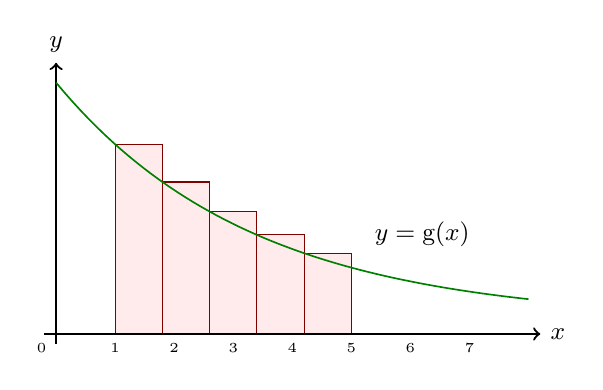
\begin{tikzpicture}[x=0.75cm,y=0.42cm,font=\small]
\foreach \k in {1,1.8,2.6,3.4,4.2}{\fill[red!8,draw=red!50!black,thin] (\k,0) rectangle ({\k+0.8},{8*exp(-0.3*\k)*0.9+0.4});}
\draw[->,thick] (-0.2,0)--(8.2,0) node[right]{$x$}; \draw[->,thick] (0,-0.3)--(0,8.2) node[above]{$y$};
\draw[green!50!black,semithick,domain=0:8,samples=60] plot (\x,{8*exp(-0.3*\x)*0.9+0.4});
\node at (6.2,3.0){$y=\mathrm{g}(x)$};
\foreach \k in {1,...,7}{\node[below,font=\tiny] at (\k,0){$\k$};}\node[below left,font=\tiny] at (0,0){$0$};
\end{tikzpicture}}
\newcommand{\figASRJC}[1]{% 0 question, 1 solution (a), 2 solution (b)
\begin{tikzpicture}[scale=0.9,font=\small]
\ifnum#1<2 \fill[gray!45] plot[domain=-2:1,samples=60](\x,{sqrt(4-\x*\x)})--plot[domain=1:-2](\x,{(\x+2)/sqrt(3)})--cycle;\fi
\ifnum#1=2 \fill[pattern=north east lines,pattern color=blue!70!black] plot[domain=1:2,samples=40](\x,{sqrt(4-\x*\x)})--(2,{4/sqrt(3)})--cycle;
\draw[densely dotted](0,{4/sqrt(3)})--(2,{4/sqrt(3)});\draw[densely dotted](0,{sqrt(3)})--(1,{sqrt(3)});\draw(2,0)--(2,{4/sqrt(3)});
\node[left] at (0,{4/sqrt(3)}){$\frac{4}{\sqrt3}$};\node[left] at (0,1.62){$\sqrt3$};\node[below right] at (2,0){$2$};\node[below left] at (0,0){$0$};\fi
\draw[->](-3,0)--(3.6,0) node[right]{$x$}; \draw[->](0,-2.6)--(0,3) node[above]{$y$};
\draw[thick] (0,0) circle (2);
\draw[thick,domain=-3.2:3.2] plot (\x,{(\x+2)/sqrt(3)}) node[right]{$\sqrt3y=x+2$};
\node at (1.7,-1.6){$x^{2}+y^{2}=4$};
\ifnum#1=0 \node[above] at (0.4,2.1){$\left(1,\sqrt3\right)$};\fi
\ifnum#1=1 \node[above] at (0.4,2.1){$\left(1,\sqrt3\right)$};\draw[densely dotted](1,0)--(1,{sqrt(3)});\node[below] at (1,0){$1$};\node[below left] at (-2,0){$-2$};\fi
\end{tikzpicture}}
\newcommand{\figTJC}{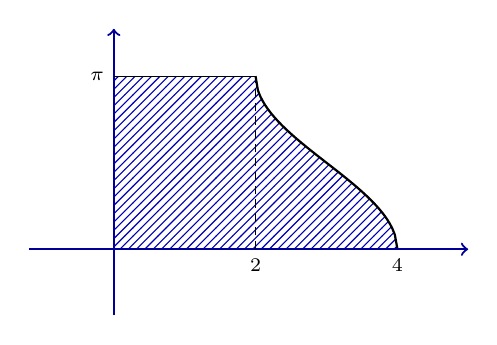
\begin{tikzpicture}[x=0.9cm,y=0.7cm,font=\small]
\fill[pattern=north east lines,pattern color=blue!70!black] (0,0)--(0,pi)--(2,pi)--plot[domain=2:4,samples=60](\x,{acos(\x-3)*pi/180})--(4,0)--cycle;
\draw[->,thick,blue!60!black] (-1.2,0)--(5,0); \draw[->,thick,blue!60!black] (0,-1.2)--(0,4);
\draw[thick] (2,pi)--plot[domain=2:4,samples=60](\x,{acos(\x-3)*pi/180});
\draw (0,pi)--(2,pi); \draw[densely dashed] (2,0)--(2,pi);
\node[left,font=\scriptsize] at (0,pi){$\pi$}; \node[below,font=\scriptsize] at (2,0){$2$}; \node[below,font=\scriptsize] at (4,0){$4$};
\end{tikzpicture}}
%% ============================================================ 121 2021 A-level P2 Q2 (soln: Raffles Institution "Solution for 2021 A-Level Paper 2", /workspace/tmp_ch10/RI_TYS_2021_AL_P2_sol.pdf pp3-4)
\defQ{121}{}{%
The diagram shows a sketch of the curve $y=\mathrm{f}(x)$. The region under the curve between $x=1$ and $x=5$, shown shaded in the diagram, is $A$. This region is split into 5 vertical stripes of equal width, $h$.
\begin{center}\figALstrips{1}\end{center}
\begin{qparts}
\pt{(a)} State the value of $h$ and show, using a sketch, that $\displaystyle\sum_{n=0}^{4}\left(\mathrm{f}\left(1+nh\right)\right)h$ is less than the area of $A$. \mk{2}
\pt{(b)} Find a similar expression that is greater than the area of $A$. \mk{1}
\end{qparts}
You are now given that $\mathrm{f}\left(x\right)=\dfrac{1}{20}x^{2}+1$.
\begin{qparts}
\pt{(c)} Use the expression given in part \textbf{(a)} and your expression from part \textbf{(b)} to find lower and upper bounds for the area of $A$. \mk{2}
\pt{(d)} Sketch the graph of a function $y=\mathrm{g}\left(x\right)$, between $x=1$ and $x=5$, for which the area between the curve, the $x$-axis and the lines $x=1$ and $x=5$ is less than $\displaystyle\sum_{n=0}^{4}\left(\mathrm{g}\left(1+nh\right)\right)h$. \mk{1}
\end{qparts}
\src{2021 A-level P2 Q2}}
\defS{121}{%
\begin{gtpart}{(a)}{2}The value of $h=\dfrac{5-1}{5}=\dfrac{4}{5}$.
\begin{center}\adjustbox{max width=\linewidth}{\figALstrips{2}}\end{center}
[ Note that
\begin{topalign}
\sum_{n=0}^{4}\left(\mathrm{f}(1+nh)\right)h&=h\mathrm{f}(1)+h\mathrm{f}(1+h)+h\mathrm{f}(1+2h)\\
&\quad+h\mathrm{f}(1+3h)+h\mathrm{f}(1+4h)
\end{topalign}
$h\mathrm{f}(1)$ represents the area of left-most rectangle in the diagram above. Similarly, $h\mathrm{f}(1+h)$ represents the area of second left-most rectangle in the diagram above, and $h\mathrm{f}(1+4h)$ represents the area of right-most rectangle in the diagram above.\par
So, $\displaystyle\sum_{n=0}^{4}\left(\mathrm{f}(1+nh)\right)h$ represents the sum of the area of the 5 shaded rectangles. Clearly, the total area of the rectangles is less than the area of $A$. ]\end{gtpart}
\begin{gtpart}{(b)}{1}A similar expression is $\displaystyle\sum_{n=1}^{5}\left(\mathrm{f}(1+nh)\right)h$ or $\displaystyle\sum_{n=0}^{4}\left(\mathrm{f}\left(1+\left(n+1\right)h\right)\right)h$\end{gtpart}
\begin{gtpart}{(c)}{2}\cmtrow[2mm]{\small Note that you can use the GC to evaluate the sum}{\begin{topalign}
\mathrm{f}(x)&=\frac{1}{20}x^{2}+1.
\end{topalign}
\begin{topalign}
\text{Lower bound for area of }A&=\sum_{n=0}^{4}\left(\mathrm{f}(1+nh)\right)h\\
&=\frac45\sum_{n=0}^{4}\left(\frac{1}{20}\left(1+\frac45n\right)^{2}+1\right)=5.608\\
\text{Upper bound for area of }A&=\sum_{n=1}^{5}\left(\mathrm{f}(1+nh)\right)h\\
&=\frac45\sum_{n=1}^{5}\left(\frac{1}{20}\left(1+\frac45n\right)^{2}+1\right)\\
&=6.568
\end{topalign}}\end{gtpart}
\begin{gtpart}{(d)}{1}\begin{center}\adjustbox{max width=\linewidth}{\figALg}\end{center}\end{gtpart}}
%% ============================================================ 122 ASRJC 2025 Prelim P1 Q7 (soln: ASRJC_2025_H2_Math_Prelim_P1_Solutions.pdf pp12-14, official)
\defQ{122}{}{%
Curve $C$ is a circle with radius 2 and center at the origin with equation $x^{2}+y^{2}=4$. Line $L$ has the equation $\sqrt3y=x+2$. The diagram below shows the shaded region $A$ which is enclosed between $C$ and $L$.
\begin{center}\figASRJC{0}\end{center}
\begin{qparts}
\pt{(a)} Use the substitution $x=2\sin\theta$ to show that the area of region $A$ can be written in the expression $\displaystyle\int_{b}^{a}4\cos^{2}\theta\,\dD\theta-c$, where $a$, $b$ and $c$ are exact constants to be determined.\par Hence evaluate this area exactly. \mk{6}
\pt{(b)} The region $B$ is bounded by the curve $C$, the line $L$ and the line $x=2$. Find the volume generated when region $B$ is rotated through $2\pi$ radians about the $y$-axis. Give your answer to two decimal places. \mk{3}
\end{qparts}
\src{ASRJC 2025 Prelim P1 Q7}}
\defS{122}{%
\begin{gtpart}{(a)}{6}\begin{center}\adjustbox{max width=\linewidth}{\figASRJC{1}}\end{center}
The circle $x^{2}+y^{2}=4$ and line $\sqrt3y=x+2$ intersects at $x=-2$ and $x=1$
\begin{topalign}
\text{Area of region }A&=\int_{-2}^{1}\sqrt{4-\left(x\right)^{2}}\,\dD x-\text{area of triangle}\\
x=2\sin\theta\quad&\Rightarrow\quad\frac{\dD x}{\dD\theta}=2\cos\theta
\end{topalign}
When $x=1\ \Rightarrow\ \theta=\sin^{-1}\left(\dfrac12\right)=\dfrac{\pi}{6}$\par
When $x=-2\ \Rightarrow\ \theta=\sin^{-1}\left(-1\right)=-\dfrac{\pi}{2}$
\begin{topalign}
&=\int_{-\frac{\pi}{2}}^{\frac{\pi}{6}}\sqrt{4-\left(2\sin\theta\right)^{2}}\left(2\cos\theta\right)\dD\theta-\frac12\left(3\right)\sqrt3\\
&=\int_{-\frac{\pi}{2}}^{\frac{\pi}{6}}\left(2\cos\theta\right)\left(2\cos\theta\right)\dD\theta-\frac{3\sqrt3}{2}\\
&=\int_{-\frac{\pi}{2}}^{\frac{\pi}{6}}4\cos^{2}\theta\,\dD\theta-\frac{3\sqrt3}{2}\ \text{(shown)}
\end{topalign}
Where $a=\dfrac{\pi}{6},b=-\dfrac{\pi}{2},c=\dfrac{3\sqrt3}{2}$
\begin{topalign}
4\int_{-\frac{\pi}{2}}^{\frac{\pi}{6}}\cos^{2}\theta\,\dD\theta&=4\int_{-\frac{\pi}{2}}^{\frac{\pi}{6}}\left(\frac{\cos2\theta+1}{2}\right)\dD\theta\\
&=2\int_{-\frac{\pi}{2}}^{\frac{\pi}{6}}\left(\cos2\theta+1\right)\dD\theta\\
&=2\left[\frac{\sin2\theta}{2}+\theta\right]_{-\frac{\pi}{2}}^{\frac{\pi}{6}}
\end{topalign}
\begin{topalign}
\text{Required area}&=2\left[\left(\frac12\sin2\left(\frac{\pi}{6}\right)+\frac{\pi}{6}\right)-\left(\frac12\sin2\left(-\frac{\pi}{2}\right)-\frac{\pi}{2}\right)\right]-\frac{3\sqrt3}{2}\\
&=\left(2\left(\frac{\sqrt3}{4}+\frac{\pi}{6}+\frac{\pi}{2}\right)\right)-\frac{3\sqrt3}{2}\\
&=\frac{\sqrt3}{2}+\frac{4\pi}{3}-\frac{3\sqrt3}{2}=\frac{4\pi}{3}-\sqrt3
\end{topalign}\end{gtpart}
\begin{gtpart}{(b)}{3}\begin{center}\adjustbox{max width=\linewidth}{\figASRJC{2}}\end{center}
Volume obtained by rotating region $B$ through $2\pi$ radians about $y$-axis
\begin{topalign}
&=\text{volume of cylinder}-\pi\int_{\sqrt3}^{\frac{4}{\sqrt3}}\left(\sqrt3y-2\right)^{2}\dD y-\pi\int_{0}^{\sqrt3}\left(4-y^{2}\right)\dD y\\
&=\pi\left(2\right)^{2}\left(\frac{4}{\sqrt3}\right)-\pi\int_{\sqrt3}^{\frac{4}{\sqrt3}}\left(\sqrt3y-2\right)^{2}\dD y-\pi\int_{0}^{\sqrt3}\left(4-y^{2}\right)\dD y\\
&\approx8.4644\\
&\approx8.46\ \text{(2 d.p.)}
\end{topalign}\end{gtpart}}
%% ============================================================ 123 TJC 2025 Prelim P1 Q10 (soln: TJC_2025_H2_Math_Prelim_P1_Solutions.pdf pp11-12, official)
\defQ{123}{}{%
\begin{qparts}
\pt{(a)} Differentiate $\sqrt{1-x^{2}}$ with respect to $x$.\par Hence evaluate $\displaystyle\int_{-1}^{1}\cos^{-1}x\,\dD x$, giving your answer in exact form. \mk{5}
\pt{(b)} The finite region $R$ is bounded by the curve $y=\cos^{-1}\left(x-3\right)$, where $2\leqslant x\leqslant4$, the line $y=\pi$ and the axes.
\begin{qparts}[2.2em]
\pt{(i)} Describe a geometrical transformation which will map the graph of $y=\cos^{-1}\left(x-3\right)$ onto the graph of $y=\cos^{-1}x$. \mk{1}
\pt{(ii)} Hence or otherwise, find the area of $R$ in exact form. \mk{2}
\end{qparts}
\pt{(c)} Find the exact value of the volume generated when $R$ is rotated completely about the $y$-axis. \mk{4}
\end{qparts}
\src{TJC 2025 Prelim P1 Q10}}
\defS{123}{%
\begin{gtpart}{(a)}{5}\begin{topalign}
\frac{\dD}{\dD x}\sqrt{1-x^{2}}&=\frac{-2x}{2\sqrt{1-x^{2}}}=-\frac{x}{\sqrt{1-x^{2}}}\\
\int_{-1}^{1}\cos^{-1}x\,\dD x&=\Big[x\cos^{-1}x\Big]_{-1}^{1}-\int_{-1}^{1}x\left[-\frac{1}{\sqrt{1-x^{2}}}\right]\dD x\\
&=1(0)-(-1)(\pi)-\int_{-1}^{1}\frac12\cdot\frac{-2x}{\sqrt{1-x^{2}}}\,\dD x\\
&=\pi-\left[\sqrt{1-x^{2}}\right]_{-1}^{1}\\
&=\pi-0\\
&=\pi
\end{topalign}\end{gtpart}
\begin{gtpart}{(b)(i)}{1}Translate the graph of $y=\cos^{-1}(x-3)$ three units in the negative direction of $x$-axis to obtain the graph of $y=\cos^{-1}x$\end{gtpart}
\begin{gtpart}{(b)(ii)}{2}\begin{center}\figTJC\end{center}
\begin{topalign}
\text{Area of the region }R&=\left(2\right)\left(\pi\right)+\int_{2}^{4}\cos^{-1}\left(x-3\right)\dD x\\
&=2\pi+\int_{-1}^{1}\cos^{-1}u\,\dD u\\
&=3\pi
\end{topalign}
Alternative Method:
\begin{topalign}
\text{Area of the region }R&=\int_{0}^{\pi}3+\cos y\,\dD y\\
&=\Big[3x+\sin y\Big]_{0}^{\pi}\\
&=3\pi
\end{topalign}\end{gtpart}
\begin{gtpart}{(c)}{4}\begin{center}\figTJC\end{center}
Volume generated when rotated completely about $y$-axis
\begin{topalign}
&=\pi\int_{0}^{\pi}x^{2}\,\dD y\\
&=\pi\int_{0}^{\pi}\left(\cos y+3\right)^{2}\dD y\\
&=\pi\int_{0}^{\pi}\left(\cos^{2}y+6\cos y+9\right)\dD y\\
&=\pi\int_{0}^{\pi}\left[\frac12\left(\cos2y+1\right)+6\cos y+9\right]\dD y\\
&=\pi\left[\frac14\sin2y+6\sin y+\frac{19}{2}y\right]_{0}^{\pi}\\
&=\frac{19}{2}\pi^{2}
\end{topalign}\end{gtpart}}
